\section{Introduction}

Explaining the operation of algorithms is a fundamental part of teaching
computer science. Instructors of courses such as introductory CS, data structures, algorithms,
and compilers often explain algorithms by sketching diagrams on the
blackboard or in PowerPoint slides~\cite{Orsega2012}. With the recent growth of
Massive Open Online Courses (MOOCs), millions of students around the world now
watch online lecture videos where instructors draw and explain these diagrams
(see \fig{fig:6006-insertion}).

Instructors find it tedious and error-prone~\cite{Ross1991} to draw diagrams on
the blackboard or create animations in PowerPoint. One alternative is to use a
programming language with GUI libraries to hand-code algorithm
animations~\cite{Shaffer2011}. These animations are interactive, but they take
even longer to create, since instructors must write code rather than directly
drawing.

Another limitation of drawn or PowerPoint diagrams is that they simply consist
of geometric shapes on a canvas, without any programming-specific affordances or
constraints. Thus, students cannot interact with the instructor's demonstrations
to ground their understanding in actual code, or practice tracing the algorithm
themselves on different input data.
% may need to add a connecting sentence here about dead shapes being bad for
% teachers, before discussing possible improvements for students.
% when watching an instructor demonstrate an algorithm, either in-person or on
% video.

\begin{figure}

\begin{center}
%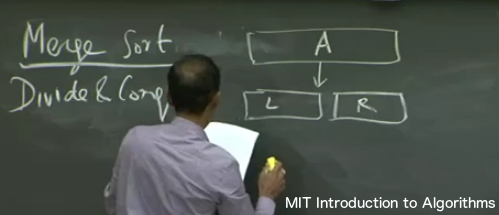
\includegraphics[width=0.55\columnwidth]{img/frontpage-6006.png}
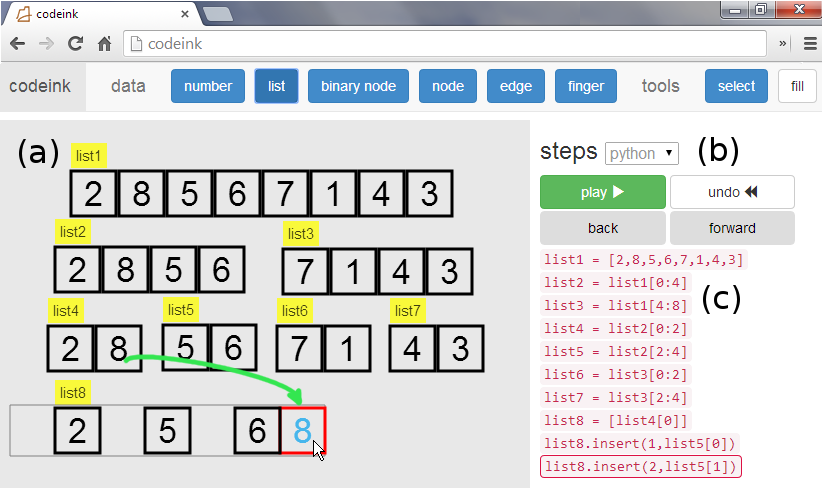
\includegraphics[width=\columnwidth]{img/frontpage-mergesort.png}
\end{center}

\vspace{-0.5em}

\caption{CodeInk is a Web-based tool that implements a direct
manipulation language for tracing algorithms on data structures for the
purpose of CS education. CodeInk allows the user to (a) compose and
manipulate data structures on a graphical canvas, (b) step forward and
backward through the recorded trace, and (c) see each step translated
into a line of Python code.}

%The CodeInk user interface is (a) a canvas for composing and
%manipulating data structures and (c) an interactive list of Python steps
%recorded by the tool, based on the user's interactions. The user can
%step forward and backward through the steps, or replay the entire trace
%using the playback controls (b).}

\label{fig:codeink-intro}
\end{figure}

To help overcome these limitations, we have developed, to our knowledge, the
first direct manipulation (DM) language for tracing the operation of algorithms
on example data structures. Specifically, the language provides a mapping from
gestures to programmatic steps on lists, binary trees, and graphs. It enables
users to trace the behavior of algorithms commonly taught in CS courses.
However, it does not yet support general iteration or conditional branching, so
it can record only concrete traces.
% at a level suitable: good way to explain that the language is about traces,
% but just comes across as ambiguous/confusing

We have also built CodeInk, a Web-based algorithm animation tool that implements
our DM language. CodeInk allows users to demonstrate an algorithm's trace on an
example by directly manipulating a visual data structure that has
programming-specific affordances and constraints. For example, an instructor can
explain merge sort by dragging an example list onto the canvas, selecting
sublists with a rectangular selection, dragging them away to create copies, then
merging elements by dragging them into a new sorted list
(\fig{fig:codeink-intro}a). Every interaction is interpreted as a step in Python
(\fig{fig:codeink-intro}c); viewers can step forward and backward through the
resulting trace (\fig{fig:codeink-intro}b).

CodeInk has three potential benefits for CS education:

\begin{itemize}\itemsep2pt

\item Instructors can easily create algorithm explanations that can be
used in class or disseminated online.

\item Students can step through instructor-created explanations to learn
both the algorithms and basic Python constructs, such as list
manipulation operators.

\item Students can solidify their understanding by tracing an algorithm on new
input data. CodeInk records all user interactions, which enables instructors to
give targeted feedback~\cite{Balzer1989} on the student's problem-solving
process.

\end{itemize}

%We evaluated CodeInk on \todo{N} teaching assistants and \todo{M}
%students in a Python-based introductory CS course at MIT.

\newpage
In this paper, we:% makes three main contributions:

\begin{enumerate} %\itemsep1pt

\item describe, to our knowledge, the first direct manipulation language
for tracing algorithms on example data structures,

\item describe CodeInk, a prototype algorithm animation tool that
implements our language,

\item and report on an empirical evaluation of CodeInk and its DM
language on students and teaching assistants in introductory CS classes.
% and discussion of the \textbf{design space} of direct manipulation languages
% for education.

\end{enumerate}

